\begin{figure}[t]
\centerline{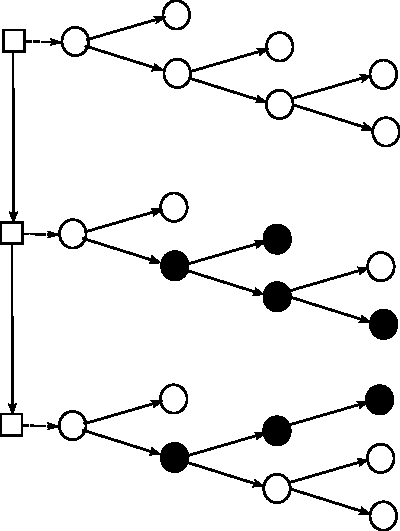
\includegraphics{fig/committree.pdf}}
\caption{A sample commit tree. In the graph, squares represent commit objects,
circles represent files or directories. The circles in black are allowed to
be accessed by a specific user. \mw{Figure not entirely clear. Question:
why do the black circles change?}}
\label{f:commit-tree}
\end{figure}

\endinput


